\documentclass[10pt]{article}
\usepackage[portuges]{babel}
\usepackage[utf8]{inputenc}
\usepackage{natbib}
\usepackage{graphicx}
\usepackage{float}

\title{Hybrid Rendering with Nau3D and OptiX}
\author{
    Leandro Salgado\\
    \texttt{A70949}
    \and
    Luís Costa\\
    \texttt{A73434}
}
\date{Departamento de Informática\\Universidade do Minho}


\begin{document}

\maketitle

\newpage

\section{Introdução} \label{sec:int}


\subsection{Motivação}~

O elevado custo de fazer \textit{render} de cenas usando \textit{raytracing} leva a que muitas vezes não seja possível fazer uso desta técnica quando o objetivo é conseguir fazer \textit{render} em tempo real. Tal acontece, por exemplo, no mundo dos jogos, em que processar dados em \textit{realtime} é essencial para que a experiência de jogo seja aceitável.

As técnicas de \textit{raytracing} atualmente utilizadas conseguem, e são, por isso, muito mais lentas, fazer \textit{render} de cenas de tal forma detalhadas que replicar esse efeito com rasterização seria, no mínimo, extremamente complicado e, no máximo, simplesmente impossível. Para além da capacidade de criar cenas com maior detalhe, o \textit{raytracing} permite simular uma série de fenómenos físicos, como reflexões especulares, cáusticas, sombras com penumbras, iluminação indireta, fluorescência, entre outros, que normalmente não são simuláveis com rasterização. A consequência de criar cenas apenas com rasterização é, muitas vezes, a inexistência de muitos fenómenos físicos e a sua consequente perceção por parte dos observadores. No caso dos jogos, a exigência na qualidade dos gráficos pelos utilizadores tem aumentado consistentemente e, consequentemente, novas formas de criar cenas com níveis de detalhe têm vindo a ser experimentadas, de forma a poder acompanhar essas exigências.

Numa tentativa de compatibilizar os benefícios de rasterização e de \textit{raytracing}, muitos jogos (talvez a maioria nos dias de hoje, pelo menos os maiores) fazem uso de vários \textit{renderers} diferentes, selecionando diferentes partes da cena e fazendo o seu \textit{render} usando diferentes técnicas.

A grande vantagem deste tipo de solução é a de possibilitar, por exemplo, fazer \textit{render} de partes da cena em que interessa simular fenómenos como reflexão especular e sombras usando \textit{raytracing} e usando rasterização para fazer \textit{render} de outras partes da cena cujo nível de detalhe não tem de ser demasiado elevado. Se for bem sucedido, este método de criar cenas beneficia, por um lado, de um aumento de performance considerável, uma vez que a rasterização, para a mesma cena, é muito mais rápida, e, por outro lado, de um aumento de detalhe e realismo, devido ao uso de \textit{raytracing}. Se a escolha de quais partes serão \textit{rendered} por quais \textit{renderers} for bem feita, os benefícios poderão ser grandes o resultado obtido poderá compensar imenso face à perda marginal de desempemnho.


\subsection{Objetivos}~

Dadas as enormes vantagens que podem surgir da utilização de \textit{renderers} híbridos, ou seja, fazer \textit{render} de cenas com \textit{renderers} diferentes, o objetivo principal deste projeto consiste essencialmente em conseguir criar uma prova de conceito do funcionamento desta estratégia, ou seja, fazer \textit{render} de uma cena utilizando rasterização e \textit{raytracing} seletivamente em \textit{realtime}, mostrando tanto as vantagens como as desvantagens ou limitações desta estratégia.

Para além da implementação em si, este projeto visa também servir como uma breve introdução à utilização do \textit{engine Nau3D} integrado com o \textit{OptiX} da \textbf{NVIDIA}. A \textit{Nau3D} é usada, para além de executar funcionalidades do \textit{OptiX}, para fazer o \textit{render} das cenas com rasterização e depois combinar os resultados com o \textit{OptiX}.

Mais concretamente, de forma a demonstrar a integração dos dois \textit{renderers} na criação de uma cena "híbrida", optamos por criar duas \textit{demos} distintas.

A primeira \textit{demo} consiste apenas na divisão da cena em duas partes iguais, em que uma das partes é criada com rasterização e a outra com \textit{raytracing}. Esta \textit{demo}, mesmo sendo simples, já demonstra que a integração da \textit{Nau3D} com o \textit{OptiX} funciona devidamente, pois significa que é possível determinar, em cada \textit{pixel}, qual o método de calcular a sua cor.

A segunda \textit{demo}, e talvez a mais interessante, consiste num \textit{rendering} mais seletivo, no sentido em que não é feita uma simples divisão da cena em duas partes, sendo antes selecionadas zonas específicas da cena que devem ser \textit{rendered} com \textit{raytracing}. Essa seleção, no caso da nossa implementação, tem a ver sobretudo com os materiais da cena, mas poderia ser feita usando outros critérios. Neste caso, optamos por tentar aplicar \textit{raytracing} nos materiais da cena que correspondam a vidros, i.e, que contenham uma forte componente especular que possa ser explorada. Usamos também \textit{raytracing} nas grades das janelas uma vez que, devido à forma como estão criadas no modelo, são opacas e, por isso, não se consegue visualizar nada que esteja atrás destas.

Na secção seguinte iremos precisar como o projeto foi implementado, explicando como funciona a integração dos dois \textit{renderers}, o \textit{pipeline} gráfico e como são combinados os dois componentes para obter o resultado final.




\section{Implementação} \label{sec:imp}

\subsection{Integração da Nau com OptiX}~
Para utilizar \textit{OptiX} em conjunto com a \textit{Nau3D}, são necessárias 3 ferramentas: \textit{Nau3D}\footnote{http://nau3d.di.uminho.pt/}, \textit{OptiX}\footnote{https://developer.nvidia.com/optix}, e \textit{Cuda 9.0}\footnote{https://developer.nvidia.com/cuda-90-download-archive}(atualmente, a \textit{Nau3D} apenas suporta a versão 9.0 de \textit{Cuda}).

\subsection{Pipeline}~
Devido a limitações das ferramentas escolhidas, foi necessário dividir a implementação em 2 \textit{demos}. Ambas as \textit{demos} seguem a mesma estrutura com 2 \textit{pipelines}, o primeiro apenas com um passo de rasterização, e o segundo com um passo de rasterização que, além de calcular a cor da cena através de rasterização, também gera uma máscara, que o passo de \textit{OptiX} utilizará para determinar onde utilizar \textit{raytracing}, seguido de um passo final que combina os resultados dos passos anteriores.

\begin{figure}[H]
    \centering
    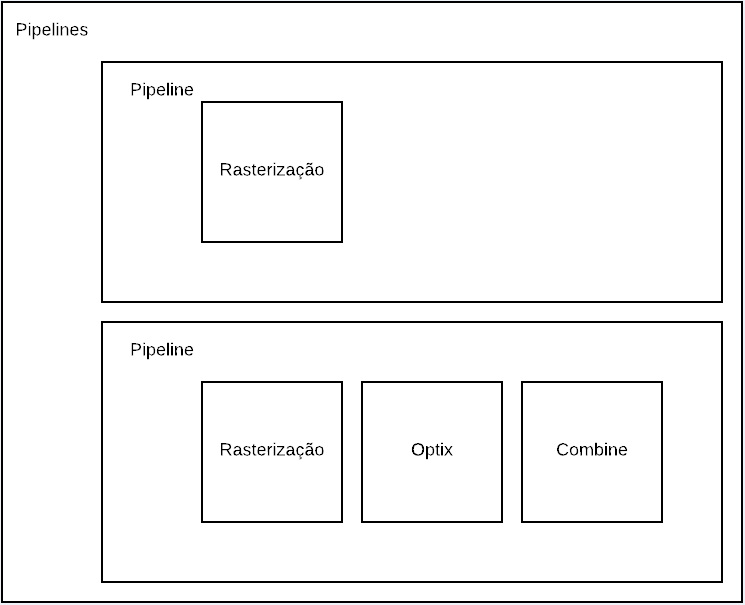
\includegraphics[width=4.7in]{estrutura.png}
    \caption{Estrutura geral das \textit{demos}}
\end{figure}

\subsection{Rasterização}~
O primeiro \textit{pipeline}, comum a ambas \textit{demos}, tem apenas uma utilização de demonstração da rasterização.

No segundo \textit{pipeline} existe um passo de rasterização, que, tal como indicado anteriormente, faz \textit{render} da cena com rasterização, e gera uma máscara. Esta máscara, no entanto, difere nas \textit{demos}.

Na \textit{demo} \textit{OptiX Half}, este passo divide horizontalmente o \textit{viewport} em 2, gerando o resultado da rasterização na metade superior, e uma máscara com informação da metade inferior da cena.

Na \textit{demo} \textit{OptiX Selective}, este passo aplica dois conjuntos de \textit{shaders} diferentes, dependendo do material da cena. A \textit{Nau3D} permite escolher que conjunto de \textit{shaders} aplicar a que materiais. Desta forma, atribuímos um conjunto de \textit{shaders}, denominado \textit{'rasters'}, aos materiais \textit{Vidro} e \textit{Grades}, e aos restantes materiais atribuímos um outro conjunto de \textit{shaders}, denominado \textit{'rastersc'}. Ambos os conjuntos de \textit{shaders} são compostos por um \textit{vertex shader} e um \textit{fragment shader}.

O conjunto de \textit{shaders} \textit{'rastersc'} é composto por um \textit{vertex shader} que apenas recolhe as informações do modelo, e do mundo, nomeadamente a posição do vértice, a sua normal, a coordenada de textura, e a direção da luz, e envia para o \textit{fragment shader}, e por um \textit{fragment shader}, que é partilhado com o conjunto de \textit{shaders} \textit{'rasters'}.

O conjunto de \textit{shaders} \textit{'rasters'} é também composto por um \textit{vertex shader}, que faz o mesmo que o \textit{vertex shader} do conjunto de shaders \textit{'rastersc'}, excepto que a direção da luz é um vector nulo. Isto pois a cor dos materiais em que este conjunto de \textit{shaders} é utilizado será calculada por \textit{raytracing} no \textit{OptiX}. Além disso, ajuda a distinguir os seus \textit{pixels} quando estes forem tratados pelo \textit{fragment shader}.

Tal como referido anteriormente, os conjuntos de \textit{shaders} \textit{'rasters'} e \textit{'rastersc'} partilham o \textit{fragment shader}. Este \textit{shader} coloca em texturas as informações de toda a cena relativas a normais e coordenadas de textura tal como recebidas dos \textit{vertex shaders}. Nesta altura, é efetuada o cálculo da cor, em que os \textit{pixels} que tenham um vetor nulo como direção da luz são colocados numa máscara, pois serão os \textit{pixels} cuja cor será calculada pelo \textit{OptiX}, enquanto que nos restantes \textit{pixels} a cor é calculada por rasterização, e o resultado é colocado na textura que depois será combinada com o resultado do \textit{OptiX}.

\subsection{Raytracing}~
No passo \textit{OptiX} é necessário indicar quais os processos que serão usados como \textit{entry point}, isto é, o processo que representa a câmara, que irá disparar os raios, e o processo a ser chamado caso seja encontrada uma exceção. É também necessário indicar os processos para interseção com a geometria, assim como os processos \textit{default} a serem chamados para os materiais. É possível também designar processos para materiais específicos, e atribuir alguns valores de \textit{input} dos vértices, como posição, normal e coordenadas de textura, assim como variáveis associadas a materiais, como as suas componentes especulares, ou outras variáveis de \textit{input}, como uma textura. É também necessário indicar onde será guardado o \textit{output} do \textit{OptiX}, seja numa textura, ou diretamente no \textit{viewport}.

Poder atribuir uma textura como valor de \textit{input} é importante, pois é assim que o \textit{OptiX} fica a conhecer a máscara gerada no passo anterior, e que lhe permite não ter de fazer \textit{render} de toda a cena.

Ao ter a máscara disponível no \textit{OptiX} como uma variável, é possível um acesso fácil a partir de qualquer processo. Em particular, a partir dos processos que representam as câmaras. Através do uso de variáveis internas do \textit{OptiX}, é possível aceder à máscara, ao \textit{pixel} que está a ser processado, e verificar as suas componentes, em especial, a 4ª componente, que permite determinar se o \textit{pixel} deverá ser ou não processado pela câmara. Em caso desta 4ª componente ter valor 0, o \textit{pixel} é "descartado", deixando no \textit{output} o \textit{pixel} a branco. Caso contrário, é calculada a direção do raio, e este é disparado.

A \textit{demo} {OptiX Half} utiliza uma câmara simples, com 1 \textit{sample per pixel}, pois é um \textit{scope} maior onde utilizar maiores \textit{samples per pixel} pode aumentar o tempo de execução, e assim reduzir as \textit{frames} por segundo.

Em contrapartida, a \textit{demo} {Optix Selective} utiliza uma câmara com \textit{multisampling}, com 16 \textit{samples per pixel}, uma vez que a área em que será calculado \textit{raytracing} é menor. Os raios são disparados aleatoriamente, utilizando uma função que gera número aleatórios presente numa \textit{library} disponibilizada pela \textbf{NVIDIA}.

Além da câmara, o processo que calcula a reflexão do vidro também deve ser mencionado. Quando o raio intercepta o vidro, é calculado o vector do raio refletido, com uma função nativa do \textit{OptiX}, e é disparado um raio nessa direção. O resultado do processo será uma multiplicação entre o resultado do raio refletido com a componente especular do material. Não foi possível adicionar refração, uma vez que iria adicionar complexidade ao processo de cálculo da luz.

\subsection{Combinação}~
Depois de obtidos os resultados do passo de rasterização e do passo de \textit{OptiX}, segue-se um passo de combinação dos resultados. Em ambas as \textit{demos}, o passo é feito utilizando o mesmo conjunto de \textit{shaders}, num passo do tipo \textit{quad}. Passos do tipo \textit{quad} são passos que preenchem o \textit{viewport} com um quadrado (dois triângulos), normalmente com o objectivo de lhe aplicar uma textura para visualização de um qualquer resultado. Um \textit{vertex shader} num passo \textit{quad} recebe como \textit{input} as coordenadas de textura associadas ao \textit{quad}, e passa-as como \textit{output} ao \textit{fragment shader}. O \textit{fragment shader}, por sua vez, recebe como \textit{input} as coordenadas de textura do \textit{quad}, e acede, nessas coordenadas, às duas texturas resultantes dos passos anteriores, e "extrai" os \textit{pixels} de ambas. Se a 4ª componente do \textit{pixel} na textura resultante do passo de rasterização for igual a 1, o \textit{fragment shader} retorna a cor desse \textit{pixel}, caso contrário, retorna a cor do \textit{pixel} extraido da textura resultante do passo de \textit{OptiX}.


\section{Obstáculos e limitações}~ \label{sec:oel}

Esta secção visa apenas identificar alguns dos problemas com que nos deparámos ao longo da implementação do projeto, bem como algumas limitações que consideramos relevantes.

Durante a implementação do projeto, houve uma série de situações que causaram dificuldades acrescidas na conclusão do projeto. Algumas das dificuldades são menos significativas e, de certa forma, até mais comuns, como é o caso da dificuldade acrescida em fazer \textit{debug} quando se trabalha em \textbf{GPU}.

Para além de compreender o funcionamento do \textit{OptiX} e de que forma este fuciona com a \textit{Nau3D} (sobre o qual tivemos alguma ajuda, inclusive com projetos já implementados aos quais tivemos acesso), o facto da única grande fonte de informação disponível \textit{online} sobre \textit{OptiX} ser a documentaação oficial da \textbf{NVIDIA} dificultou um pouco o processo. No entanto, isso contituiu apenas um pequeno obstáculo.

Devido à forma como a \textit{Nau3D} está integrada com o \textit{OptiX}, não é possível, num dado projecto, fazer mais do que um passo \textit{OptiX}, mesmo em \textit{pipelines} diferentes, pelo que qualquer \textit{demo} que seja implementada tem sempre essa limitação. Embora não tenha sido um objstáculo no caso deste projeto, pois a solução não passou por ter vários passos \textit{OptiX}, um projeto que precise de o fazer terá essa limitação.

A cor dos objetos refletidos no vidro é ligeiramente diferente da cor dos objetos originais, uma vez que os refletidos tiveram a sua cor calculada com \textit{raytracing} pelo \textit{OptiX} e os originais pela rasterização. Essa diferença, embora não seja atenuada neste projeto, é referenciada na secção \ref{sec:cetf}.

Foi também difícil utilizar o \textit{OptiX} para calcular as sombras, ao mesmo tempo que se calculam as reflexões, uma vez que isso requeriria fazer \textit{render} de toda a cena, e depois detetar as sombras na textura resultado, o que derrotaria o objetivo do \textit{render} híbrido.

\section{Resultados Obtidos}~

Esta secção tem como objetivo mostrar o resultado da implementação descrita na secção \ref{sec:imp}.

A imagem que se segue mostra o resultado de usar \textit{raytracing} com reflexão nos vidros na parte inferior da \textit{viewport} e de rasterização na parte superior. A cor dos vidros foi calculada usando 1 \textit{sample per pixel}, o que é visível na quantidade elevada de ruído na imagem.


\begin{figure}[H]
    \centering
    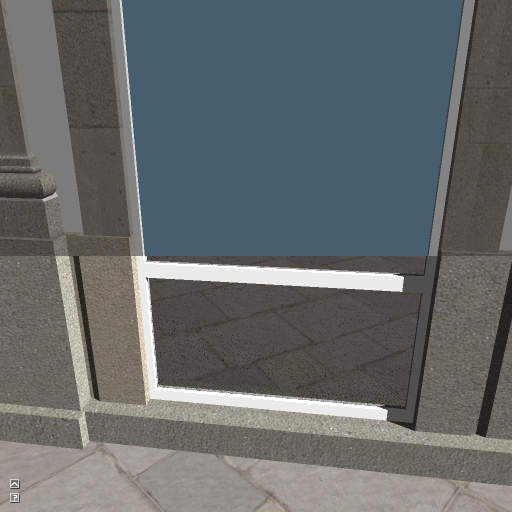
\includegraphics[width=2.5in]{half_1rpp.jpg}
    \caption{Exemplo com metade do \textit{viewport} com rasterização e a outra com \textit{raytracing} com 1 spp}
\end{figure}

A imagem seguinte mostra o resultado de aplicar \textit{raytracing} nos vidros e nas grades.

\begin{figure}[H]
    \centering
    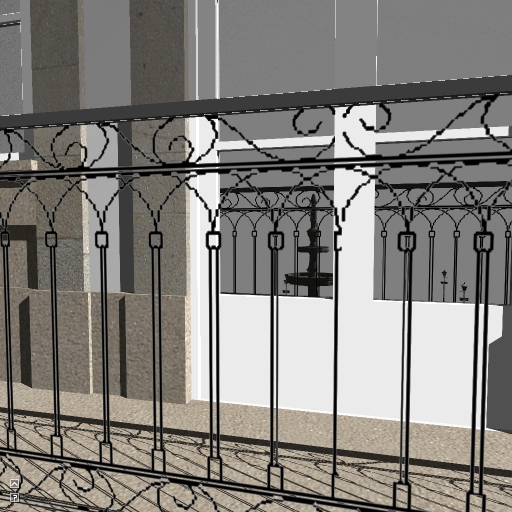
\includegraphics[width=3.3in]{reflections.jpg}
    \caption{Exemplo de janela e grades com \textit{raytracing}}
\end{figure}

Como se pode ver, mesmo sendo a geometria das grades opaca, é possível ver através destas, uma vez que a textura que está mapeada na geometria tem zonas com o valor $\alpha$ a 0. Esse valor é testado no \textit{OptiX}.Se for 0, o raio continua, se for 1, o raio interceta e termina. No entanto, é possível notar que a parede que é vista através das grades tem uma cor diferente da que é vista acima, sendo um pouco mais clara. Isso acontece porque a parece que está atrás da grade tem a sua cor calculada com \textit{raytracing}, já que os raios que a intersetam correspondem aos raios que passaram no \textit{alpha test}, i.e., que intersetaram a grade em partes cuja textura tinha o componente $\alpha$ a zero.

Este fenómeno está relacionado com o fenómeno da cor refletida ser diferente da cor dos objetos originais, uma vez que também resulta do cálculo da cor do mesmo tipo de material (ou até do mesmo objeto).

Uma vez que fazer \textit{sample} com apenas um raio por \textit{pixel} normalmente cria muito ruído na cena, fizemos a experiência de fazer \textit{render} da cena com 4 raios por \textit{pixel}, 16 raios por \textit{pixel} e 64 raios por \textit{pixel}.

As imagens seguintes representam esses três casos, respetivamente.



\begin{figure}[H]
    \centering
    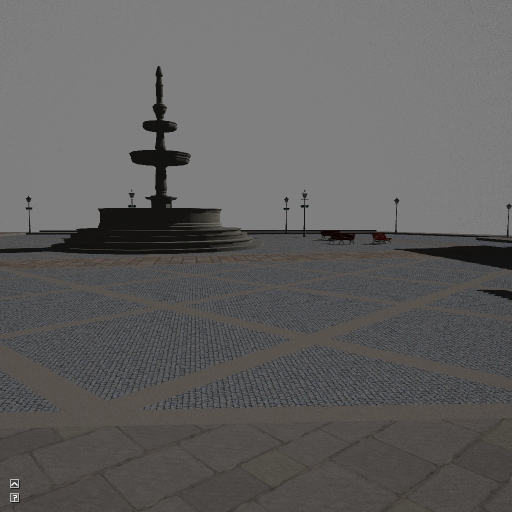
\includegraphics[width=3.3in]{selective_multisampling_4rpp_reflections.jpg}
    \caption{Exemplo de multisampling com 4 spp (só vidro)}
\end{figure}

\begin{figure}[H]
    \centering
    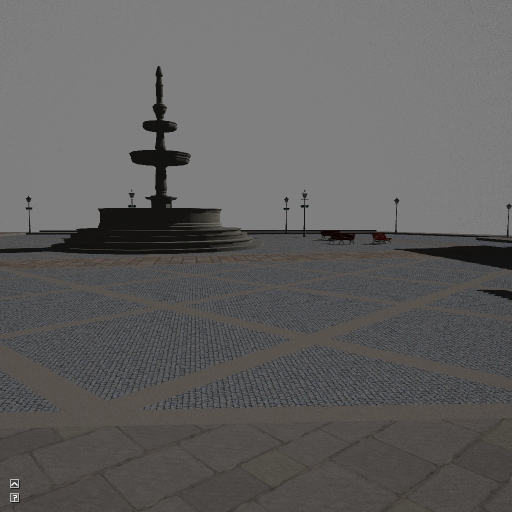
\includegraphics[width=3.3in]{selective_multisampling_16rpp_spec.jpg}
    \caption{Exemplo de multisampling com 16 spp (só vidro)}
\end{figure}

\begin{figure}[H]
    \centering
    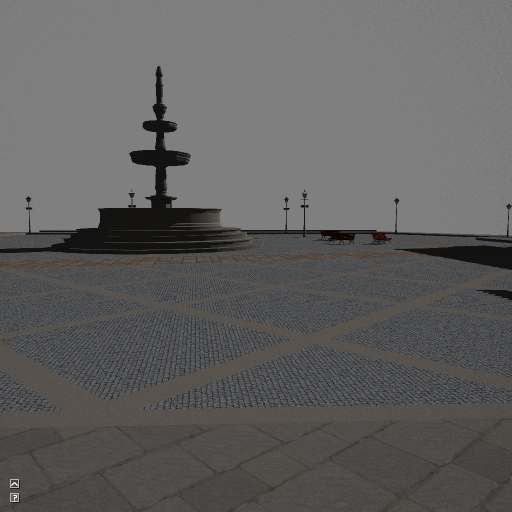
\includegraphics[width=3.3in]{selective_multisampling_64rpp.jpg}
    \caption{Exemplo de multisampling com 64 spp (só vidro)}
\end{figure}

Embora haja mudanças no desempenho quando se usa mais \textit{samples per pixel}, o aspeto resultante de usar 4, 16 ou 64 é paraticamente idêntico, pelo menos nestas imagens, pelo que não justifica que seja usado \textit{multisampling} com muito mais do que 4 \textit{samples per pixel}.

Por fim, a imagem seguinte mostra a praça de um ponto de vista mais longe. É possível ver a reflexão da fonte ao fundo, no edifício à beira do edifício com a porta verde.

\begin{figure}[H]
    \centering
    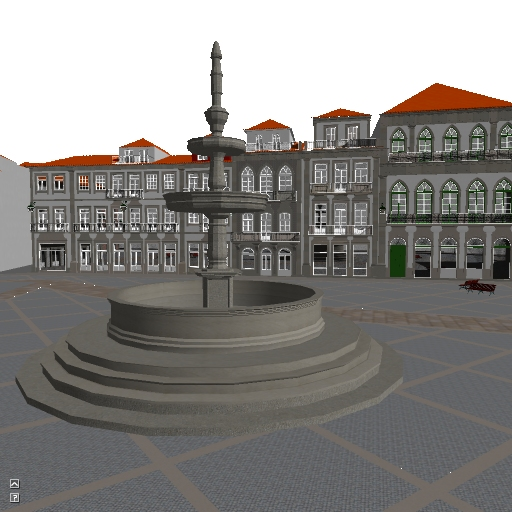
\includegraphics[width=3.5in]{scene_and_reflection.jpg}
    \caption{Imagem da praça de Ponte de Lima}
\end{figure}



\section{Considerações e Trabalho Futuro}~ \label{sec:cetf}

Embora a demonstração das capacidades da \textit{Nau3D} em conjunção com o \textit{OptiX} de fazer \textit{rendering} híbrido tenham sido demonstradas com sucesso neste projeto, as potencialidades deste método vão muito além do que foi feito nas \textit{demos} criadas.

Qualquer fenómeno físico da luz mencionado na introdução do projeto que possa ser simulado usando \textit{raytracing} pode, teoricamente, ser simulado na \textit{Nau}, embora sempre com a consciência das limitações que essas simulações possam ter.

Por exemplo, como já foi referido, fazer sombras de forma seletiva apenas com \textit{raytracing} é uma tarefa bastante mais complexa do que implementar a reflexão nos vidros, assumindo que estas não são primeiro feitas com rasterização, recorrendo a métodos como \textit{shadow maps} ou \textit{shadow volumes}. Caso haja sombras desta forma, algo que pode ser feito com \textit{raytracing} é o cálculo das penumbras. Regra geral, as sombras calculadas com rasterização sofrem de \textit{aliasing}, no sentido em que, num dado \textit{pixel}, ou há sombra e, portanto, este tem cor preta, ou não há e tem a cor do objeto representado. Em dois píxeis adjacentes, se um estiver em sombra e o outro não, a mudança é demasiado drástica e nota-se claramente os dois píxeis na borda.

Se usarmos \textit{raytracing} para calcular as sombras, a única zona em que faz sentido aplicar esta técnica é nas bordas das sombras, já que nas zonas em que há mesmo sombra a cor é preta e, portanto, não faz diferença se esta é calculada com rasterização ou com \textit{raytracing} (assumindo que não estamos a tentar calcular ilumincação indireta). Para podermos fazer \textit{raytracing} nas bordas, uma forma de o fazer seria conseguir criar uma máscara, de forma análoga ao que foi feito para detetar vidros e grades, que conseguisse detetar quais os píxeis que pretencem à borda. Logicamente, esta técnica não poderia ser feita da mesma forma que foi feita a seleção dos vidros e grades, já que as sombras não são um material.

A seleção das zonas de penumbra, e correspondente \textit{rendering}, embora não seja necessariamente muito complexa, não é evidente, pois teria, em primeiro lugar, de ser usado um critério para determinar se um determinado \textit{pixel} está em penumbra (por exemplo, verificar, dos oito píxeis à volta, se metade ou mais está em sombra) e, em segundo lugar, essa verificação teria provavelmente de recorrer ao uso de texturas que tivessem as cores dos píxeis todos da cena, calculadas num passo anterior, de forma a poder ter acesso, aquando do processamento de um \textit{pixel}, às informações dos píxeis adjacentes. Isso não só seria mais complexo de implementar, como implicaria que se fizesse \textit{render} da cena toda com rasterização antes de se poder começar a criar a máscara que iria alimentar o \textit{OptiX}, percorrendo os píxeis todos uma segunda vez.

Para além de fazer \textit{render} seletivo recorrendo a diferenciações por materiais ou por sombras, também poderia ser implementado um projeto que fizesse a seleção das zonas a fazer \textit{render} com base na distância à câmara (zonas mais próximas têm mais detalhe e, por isso, poderiam ser criadas com \textit{raytracing}) ou na distância ao centro da janela. Em jogos de \textit{First Person}, a concentração de um jogador é "puxada" continuamente para o centro do ecrã, pois é onde se situa grande parte da ação. Tendo isso em mente, pode ser boa ideia concentrar mais esforço computacional para fazer \textit{render} com mais detalhes nas zonas que são de facto mais percecionadas pelos jogadores, e colocar menos detalhe no resto da cena. Como a visão lateral humana tem baixa resolução, a falta de detalhe, nessas circunstâncias, pode não ser grave. Se houver, no entanto, movimentos bruscos na cena, essa estratégia pode falhar, pois a atenção do jogador é virada para os cantos da janela, que são cobertos pela visão periférica, que deteta muito bem movimentação rápida.

De qualquer das formas, podia ser implementada uma estratégia que aplicasse \textit{raytracing} no centro do ecrã, ou nas proximidades da câmara, e rasterização noutras partes menos importantes, tendo sempre em consideração que teria provavelmente de se encontrar uma forma de fazer com que as variações entre os dois métodos fossem suaves, ou seja, que não fosse notória a divisão entre zonas com \textit{raytracing} e zonas com rasterização.

Outra questão que importa salientar é a do critério de escolha para a máscara usada no projeto. Na implementação que temos, a escolha de quais os píxeis a processar com \textit{OptiX} vem da deteção de qual é o material que está nesse mesmo \textit{pixel}. Como usamos um \textit{shader} diferente para processar os pontos que fazem parte dos materiais que serão \textit{rendered} com \textit{raytracing}, não estamos a ter qualquer tipo de consideração sobre quais as propriedades dos materiais em \textit{runtime}, ou seja, a escolha é feita antes de correr o programa.

Poderiamos ter escolhido uma estratégia diferente que consistia em ter apenas um \textit{shader} que processasse todos os pontos do modelo e depois fazer uma seleção de quais os píxeis que seriam processados no \textit{OptiX} e quais seriam processados com rasterização com base, por exemplo, na constante de especularidade do material, sem saber exatamente que tipo de material é. Por exemplo, poderíamos usar um critério em que materiais com uma componente de especularidade acima dos 40\% seriam \textit{rendered} com \textit{raytracing}, pois a componente especular é suficientemente alta para poder fazer a diferença (os 40\% são apenas um exemplo arbitrário). Ao aplicar esta estratégia, incorreríamos na possível desvantagem de não sabermos exatamente que materiais poderíamos estar a escolher, aplicando a mesma regra a todos os que respeitassem o critério. Por outro lado, assumindo que há vários materiais com diferentes níveis de especularidade, é vantajoso ter uma solução que não tem em atenção os materiais mas sim as suas propriedades, resultando na não necessidade de especificar cada material.

Se, pelo contrário, usarmos a estratégia que foi aplicada neste projeto de definir quais os materiais a serem processados, enquanto que incorremos na necessidade de descriminar os diferentes tipos de materiais que queremos, podemos identificar materiais diferentes com propriedades muito diferentes que serão todos processados com \textit{raytracing}, algo que só poderia ser feito com conjunção de vários critérios se fosse feito com a estratégia referida anteriormente. Foi devido a ser mais fácil processar vidros e grades em conjunto e ao facto de apenas aplicarmos \textit{raytracing} a dois materiais que optamos por usar esta estratégia.

Finalmente, é possível notar claramente que os objetos da cena refletidos nos vidros são diferentes dos objetos da cena, como se viu na secção dos resultados. De facto, a cor que se vê refletida não é a mesma da cor da cena original. Isso deve-se à forma como as cores são calculadas na \textit{Nau3D} com rasterização e no \textit{OptiX} com \textit{raytracing}. A forma de mudar isso passaria por aplicar técnicas como \textit{tonemapping} para corrigir a cor refletida.

Finalmente, como foi identificado na secção \ref{sec:oel}, o problema das cores diferentes nos materiais refletidos quando comparados com as suas cores originais poderia ser resolvido utilizando técnicas como \textit{tonemapping}. Embora não tenha sido algo implementado neste projeto, devido não só à complexidade da solução, mas também ao facto de já não fazer parte do objetivo que foi delineado desde o início, esta correção das cores poderia ser feita como trabalho futuro.

\newpage


\section{Conclusão}~ \label{sec:con}
Neste projeto os objetivos gerais consistiam em introduzir a integração da \textit{Nau3D} com o \textit{OptiX} e fazer uso dessa integração para realizar uma prova de conceito de \textit{rendering} híbrido.

O programa, para um nível aceitável de \textit{samples per pixel}, executa a um nível aceitável de \textit{frames per second}, o que é especialmente bom tendo em conta que um dos grandes objetivos de fazer \textit{rendering} híbrido é o de conseguir obter resultados usando \textit{raytracing} em tempo real.

A escolha do projeto em específico pelo grupo foi tentar implementar \textit{raytracing} seletivo nos vidros de uma cena para que se pudesse observar a reflexão de vários objetos dessa cena.

Como foi mencionado na secção \ref{sec:cetf}, há uma miríade de possibilidades e possíveis implementações que podem ser feitas, que ilustram os mais variados casos de aplicação desta técnica.

\bibliographystyle{plain}
\bibliography{references}

\end{document}
